\documentclass{article}

\usepackage{tikz}

\author{Yeoun Chan Kim \and John Strauser \and Xuanang Wang}

\title{CS440 Report}

\begin{document}

\maketitle

\section*{Part 1}

\begingroup
\centering

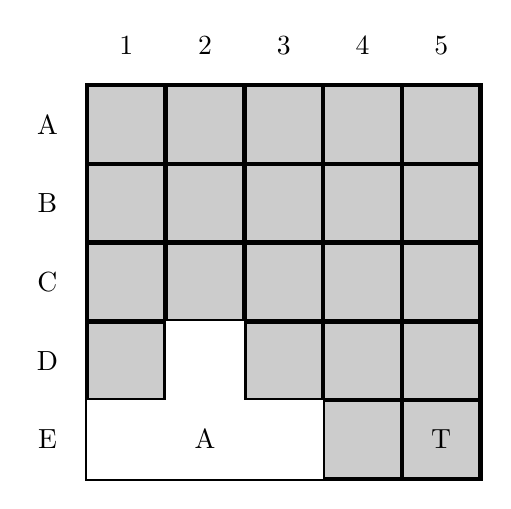
\begin{tikzpicture}
\draw [ultra thick, draw=black, fill=black!20!white] (0,0) grid  (5,5) rectangle (0,0);
\fill[white] (0,0) rectangle(1, 1);
\fill[white] (1,0) rectangle(2, 1); 
\fill[white] (2,0) rectangle(3, 1); 
\fill[white] (1,1) rectangle(2, 2); 
\node at (+1.5,+0.5) {A};
\node at (+4.5,+0.5) {T};
\node at (-0.5,+0.5) {E};
\node at (-0.5,+1.5) {D};
\node at (-0.5,+2.5) {C};
\node at (-0.5,+3.5) {B};
\node at (-0.5,+4.5) {A};
\node at (+0.5,+5.5) {1};
\node at (+1.5,+5.5) {2};
\node at (+2.5,+5.5) {3};
\node at (+3.5,+5.5) {4};
\node at (+4.5,+5.5) {5};
\end{tikzpicture}

\endgroup

\vspace{5mm} %5mm vertical space

a) Given the illustration above, we want to explain why the first move of the agent A is to the east rather than the north. Grey represents what agent cannot see and the white represents what agent can. According to the question, T is the goal state. So we calculate the Manhattan distance from A to T, which is 3 in the current situation, as h


\end{document}